Il modello descritto nella sezione \ref{Sec:problem} è stato realizzato tramite un diagramma Scicos, utilizzando SMCube per modellare processori, bus e coordinatore dei bus. In figura \ref{Fig:model_ep} è mostrato il diagramma relativo al caso Equal Priority, mentre la figura \ref{Fig:model_fp} rappresenta il modello Fixed Priority. Ovviamente, i due modelli sono del tutto identici a parte per come viene gestita la coda delle richieste che arrivano al coordinatore.

\begin{figure}
\vspace{-3cm}
\centerline{
	\begin{subfigure}[t]{1.4\textwidth}
		\centering
		\includegraphics[angle=-90, width=\textwidth]{model_ep.eps}
		\caption{Diagramma del modello Equal Priority.}
		\label{Fig:model_ep}
	\end{subfigure}
}
\centerline{
	\begin{subfigure}[t]{1.4\textwidth}
		\centering
		\includegraphics[angle=-90, width=\textwidth]{model_fp.eps}
		\caption{Diagramma del modello Fixed Priority.}
		\label{Fig:model_fp}
	\end{subfigure}
}
\caption{I due modelli implementati: Equal Priority \subref{Fig:model_ep} e Fixed Priority \subref{Fig:model_fp}. In grigio sono evidenziati i blocchi che costituiscono la coda di priorità.}
\label{Fig:models}
\end{figure}

È importante evidenziare due decisioni di progetto che sono state prese nella rappresentazione del modello:

\begin{enumerate}
\item \textbf{Disporre i bus secondo una topologia ad anello orientato}. Il motivo di questa scelta deriva da un controllo che Scicos effettua in fase di compilazione del modello per rilevare \textsl{loop algebrici}, ossia cicli di input e output potenzialmente infiniti che portano al fallimento della simulazione (figura \ref{Fig:alg_loop}). È quindi necessario aggiungere un elemento di ritardo qualora due blocchi debbano comunicare reciprocamente (o un blocco utilizzi una sua risposta come input, come accade nell'esempio di figura \ref{Fig:alg_loop_solved}). Questo significa che, nel caso di una struttura lineare come quella mostrata in figura \ref{Fig:2pc}, ogni messaggio della seconda fase del protocollo subirebbe un ritardo di un colpo di clock, rendendo la complessità temporale del protocollo lineare rispetto al numero di nodi. Con una struttura ad anello orientato, invece, occorre inserire un blocco ritardo soltanto tra due bus. La configurazione ottimale prevede il ritardo tra l'ultimo bus dell'anello (ossia quello che precede il coordinatore del 2PC) ed il coordinatore: così facendo, in un colpo di clock viene deciso quale bus soddisferà la richiesta e nel secondo colpo di clock viene raggiunta conoscenza comune.
\item \textbf{Separare la logica del coordinatore del 2PC da quella dei bus}. In questo modo tutti i bus hanno lo stesso comportamento, evitando di dover differenziare la logica del bus coordinatore da quella degli altri. Inoltre, l'automa a stati finiti di un coordinatore \textquotedblleft semplice\textquotedblright{} è ovviamente meno complesso di quello di un coordinatore che è anche un bus, diminuendo quindi la possibilità di errori in fase di implementazione. Il costo da pagare è soltanto l'aggiunta del nodo coordinatore all'interno dell'anello dei bus.
\end{enumerate}

\begin{figure}
\makebox[\textwidth][c]{
	\begin{subfigure}[t]{.5\textwidth}
		\centering
		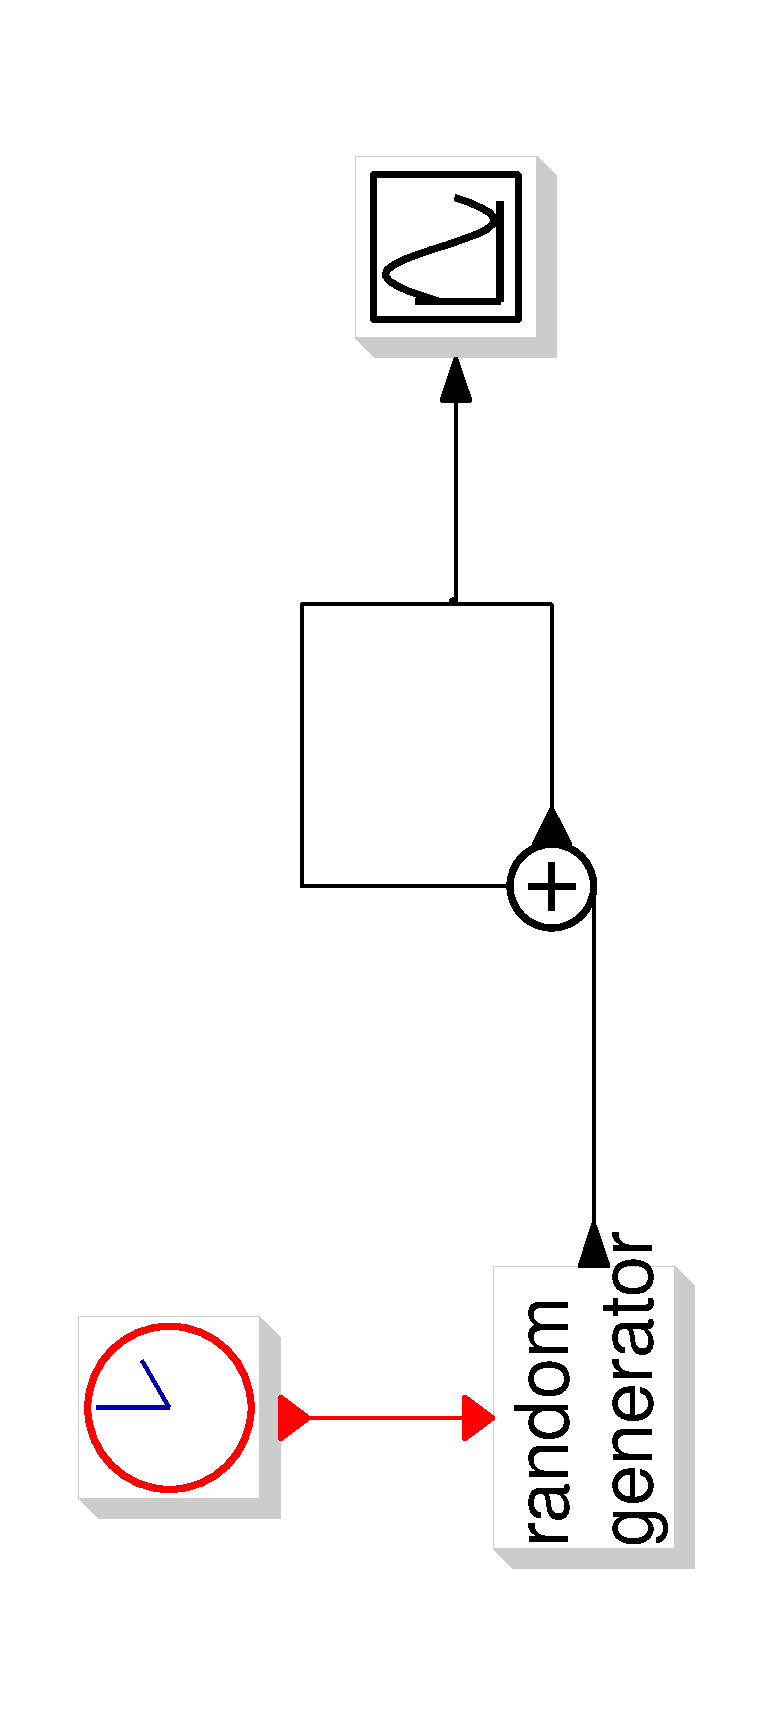
\includegraphics[angle=-90, totalheight=.45\textwidth]{alg_loop.eps}
		\caption{}
		\label{Fig:alg_loop}
	\end{subfigure}
	
	\begin{subfigure}[t]{.5\textwidth}
		\centering
		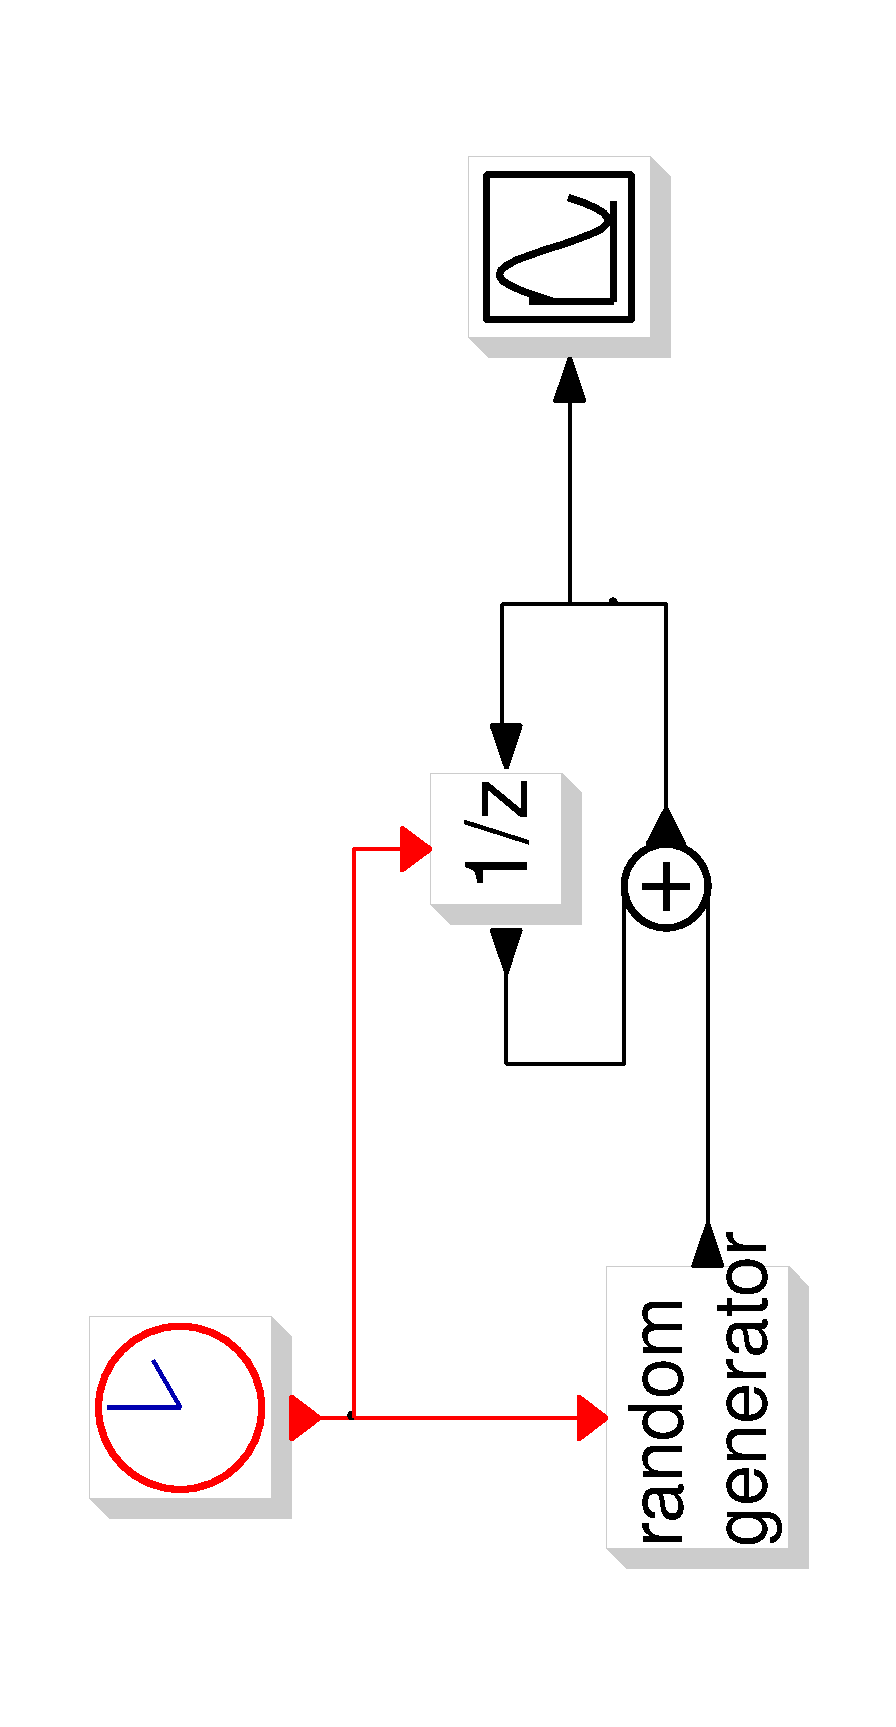
\includegraphics[angle=-90, totalheight=.45\textwidth]{alg_loop_solved.eps}
		\caption{}
		\label{Fig:alg_loop_solved}
	\end{subfigure}
}
\caption{La figura \subref{Fig:alg_loop} mostra un diagramma Scicos che contiene un loop algebrico, mentre in figura \subref{Fig:alg_loop_solved} è raffigurato un diagramma equivalente che risolve il problema inserendo un blocco ritardo.}
\label{Fig:loops}
\end{figure}

\noindent
Il modello è costruito per via grafica ed è abbastanza autoesplicativo: è facile vedere come i processori, il coordinatore ed i bus sono collegati tra di loro. Vale la pena però porre l'attenzione sugli switch antecedenti ai bus che filtrano gli output dei processori. Mentre per effettuare la richiesta i processori comunicano di fatto solo con il coordinatore, una volta garantito l'accesso la comunicazione con i bus avviene per via diretta, per evitare di aggiungere ulteriore carico di lavoro al coordinatore e rallentare le comunicazioni. Questo vuol dire che tutti i processori sono collegati a tutti i bus, ma \textit{non} è vero che tutti i segnali inviati dai processori arrivano a tutti i bus: ogni bus, infatti, controlla il proprio switch in modo che solo i segnali inviati dal processore che ha l'accesso possano arrivare.\\

Nel seguito descriveremo gli automi che modellano i processori, i bus e il coordinatore dei bus.

\subsection{Processore} 
L'automa del processore è riprodotto in figura \ref{Fig:proc_fsm}. È funzionalmente equivalente a quello riportato nelle specifiche e mostrato in figura \ref{Fig:uml}. Da notare che il tempo di soggiorno negli stati \texttt{Idle} e \texttt{Using} è random e viene campionato al momento dell'entrata nello stato.

\begin{figure}
\vspace{-1cm}
\centerline{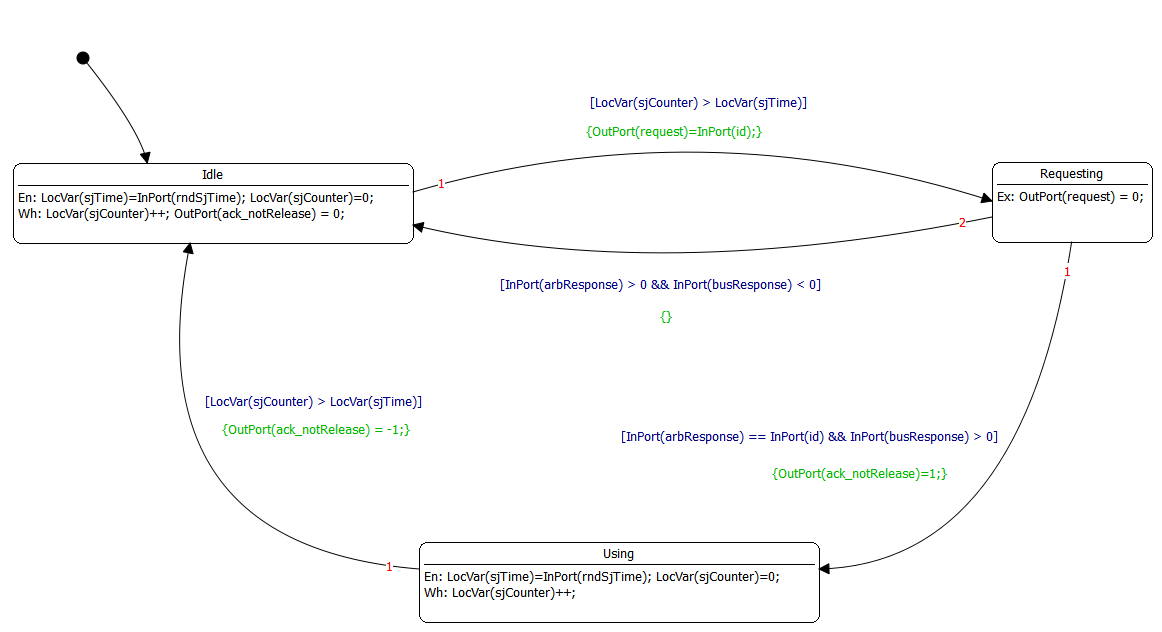
\includegraphics[width=1.4\textwidth]{processor.png}}
\caption{ASF di un processore.}
\label{Fig:proc_fsm}
\end{figure}

\pagebreak

\subsection{Coordinatore dei bus} 
L'automa del coordinatore viene mostrato in figura \ref{Fig:coord_fsm}. È composto da tre stati:

\begin{itemize}
\item \texttt{Idle}: il coordinatore è in attesa di richieste da parte dei processori.
\item \texttt{NotifyingBuses}: è arrivata una richiesta ed è stata inoltrata ai bus, dando via alla prima fase del 2PC. Il coordinatore è in attesa di sapere quale bus ha accolto la richiesta.
\item \texttt{Committing}: la richiesta è passata per tutti i bus dell'anello, tornando al coordinatore. Questo significa che a tutti i bus è arrivata la notifica della richiesta e sono tutti in attesa del commit. Il messaggio che arriva al coordinatore contiene l'id del bus che soddisferà la richiesta (o -1 se non ci sono bus disponibili) e il coordinatore non deve fare altro che inoltrarlo sia ai bus che ai processori. Quando il messaggio percorre tutto l'anello e ritorna al coordinatore, tutti i bus e i processori sono stati notificati del risultato della richiesta e il coordinatore può tornare nello stato di \texttt{Idle}.
\end{itemize}

\pagebreak

\begin{figure}
\vspace{-2cm}
\centerline{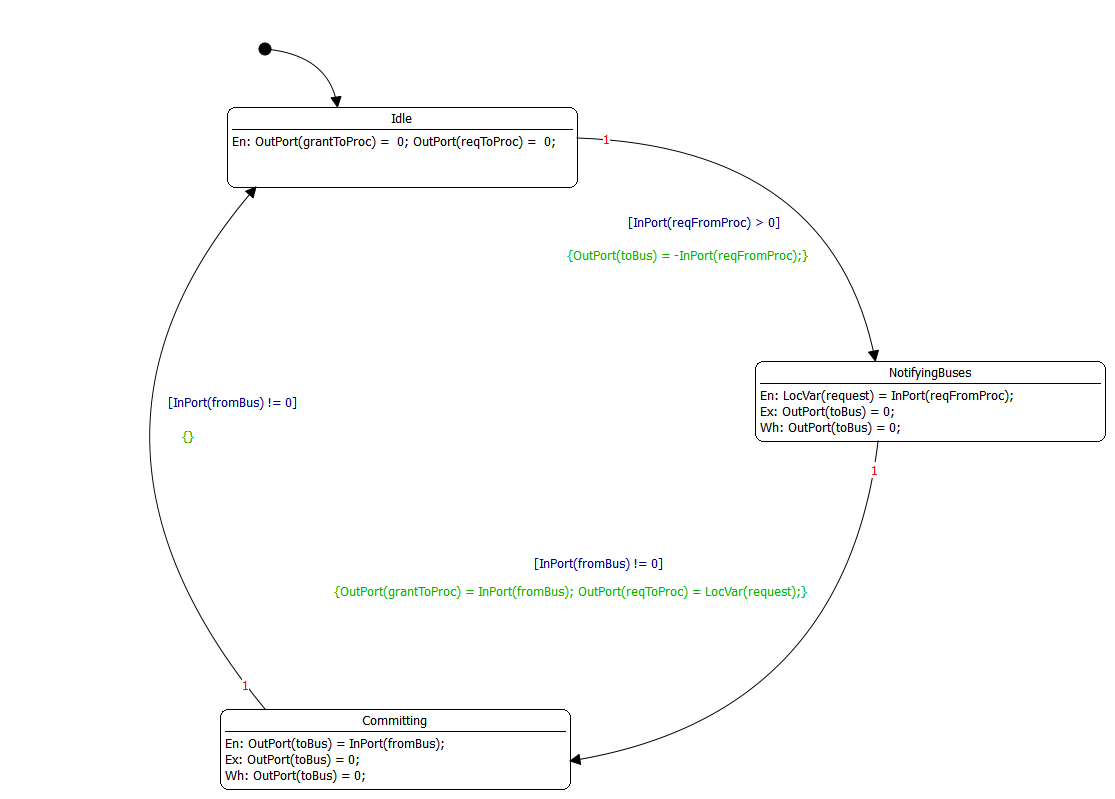
\includegraphics[width=1.4\textwidth]{busCoord.png}}
\caption{ASF del coordinatore dei bus.}
\label{Fig:coord_fsm}
\end{figure}

\subsection{Bus} 
I bus sono caratterizzati dall'ASF riportato in figura \ref{Fig:bus_fsm}. Rispetto alla macchina di figura \ref{Fig:uml} sono presenti stati aggiuntivi, derivanti dalla necessità di poter eseguire il 2PC e di doverlo fare sia mentre il bus è \texttt{Idle} che mentre serve un processore (stato \texttt{Serving}). \\


Gli stati \texttt{Idle} e \texttt{Committing} sono i due stati necessari per il funzionamento del 2PC. 

Inizialmente, il bus è \texttt{Idle}. Quando arriva una richiesta il bus entra nello stato \texttt{Committing}. Questo passaggio di stato può essere effettuato in due modi possibili: se in esso viene comunicato che la richiesta è già stata accolta, inoltrando semplicemente il messaggio; altrimenti, comunicando di incaricarsi della richiesta. Quando il messaggio compie il giro dell'anello e ritorna al bus, il 2PC è (localmente) completato e il bus può uscire dallo stato di \texttt{Committing}, andando nello stato \texttt{WaitingForProc} se deve servire il processore o tornando nello stato \texttt{Idle} se è stato invece un altro bus ad accogliere la richiesta.\\


Nello stato \texttt{WaitingForProc} il bus è in attesa del segnale \texttt{ack} da parte del processore che deve servire. Da notare che in questo stato il bus \textit{non} può prendere parte al 2PC. Questo però non è necessario, in quanto il sistema modellato è sincrono ed esente dai guasti: il segnale \texttt{ack} viene inviato dal processore e ricevuto dal bus prima che un ulteriore richiesta possa essere processata dal coordinatore. Una volta ricevuto il segnale \texttt{ack} il bus può servire il processore, passando allo stato \texttt{Serving}.\\


In linea di principio, un bus rimane \texttt{Serving} fino a quando non riceve un segnale \texttt{release} dal processore, ritornando conseguentemente nello stato \texttt{Idle}. Questo meccanismo è reso più complicato dalla necessità del bus di dover eseguire il 2PC anche mentre serve un processore, per evitare il blocco delle comunicazioni.

Se un 2PC viene iniziato mentre il bus sta servendo un processore, la richiesta non può essere localmente accolta: l'unica azione che il bus può eseguire è quella di ritrasmettere il messaggio nell'anello (\textit{relaying}), passando quindi nello stato \texttt{ServingAndRelaying}. Una volta che la prima fase del 2PC viene portata a termine e arriva il messaggio della seconda fase, il processore può tornare nello stato \texttt{Serving}.

Lo stato \texttt{Relaying} e le altre transizioni uscenti dagli stati \texttt{Serving} e \texttt{\justify ServingAndRelaying} sono necessarie per gestire i casi in cui il processore rilascia il bus prima che il 2PC venga portato a termine.

\begin{figure}[t]
\vspace{-2cm}
\centerline{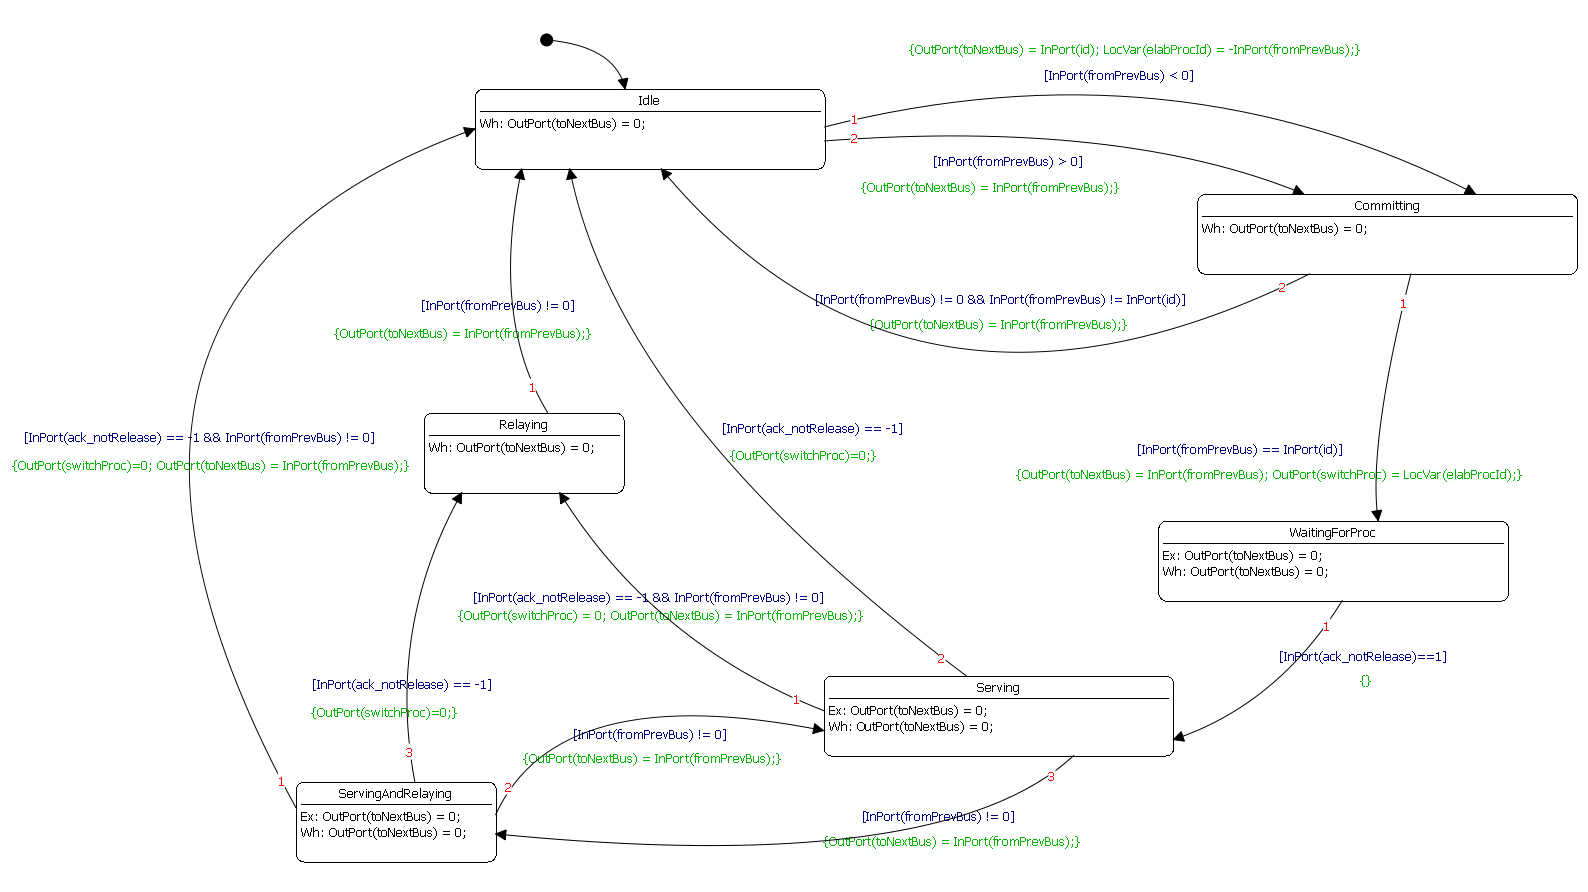
\includegraphics[width=1.6\textwidth]{bus.png}}
\caption{ASF dei bus.}
\label{Fig:bus_fsm}
\end{figure}
